\documentclass{IEEEtran}

\usepackage[utf8]{inputenc}
\usepackage{graphicx}
\usepackage[spanish]{babel}
\usepackage{authblk}
\usepackage[export]{adjustbox}
\usepackage[T1]{fontenc}
%\usepackage{url}
\usepackage{hyperref}
\usepackage{wrapfig}

\begin{document}

	\title{Cuide a su bebé, monitoree el ambiente con Arcangel}
	\author{Autores: Juan Alvares y Diego Bertolini}
	\affil{Tutor: Gabriel Taboada}
	\affil{Facultad de Ingeniería, Universidad de Palermo}
	\date{Mayo de 2018}	
	\maketitle
	
	\begin{abstract}
		Los avances tecnológicos de hoy en día prestan facilidades tanto a los consumidores como a los inventores. Diferentes herramientas están a la espera de una idea que las combine para formar un producto que solucione un problema.
        Arcangel es un dispositivo integrado a una cuna que permite monitorear a un bebé el ambiente donde se encuentra a través de distintos sensores. Entre ellos, encontramos sensores de movimiento, temperatura y humedad ambiente, sonido, luz y gases tóxicos entre otros. 
        La medición de variables ambientales en combinación con pequeños datos del bebé, nos permiten alertar a los responsables de su cuidado sobre situaciones que de otra forma pasarían desapercibidas.
	\end{abstract}
	
	Palabras clave: Bebe, Arduino, Ambiente, Sensores
	
	Nomenclaturas: App, Arduino

	\section{Introducción}
	
		\fontfamily{pcr}
	
		El cuidado de bebés es un proceso altamente demandante en tiempo para las personas a cargo. La tarea incluye el monitoreo del propio bebé así como del ambiente donde se encuentra. 
Existen tecnologías de avanzada, con márgenes de error muy pequeños que se usan a diario en medicina. No pretendemos competir con esos productos, sino utilizar tecnología más simple y accesible para solucionar problemas cotidianos a la hora de cuidar bebés.
Si bien la tecnología nos permite obtener datos médicos como el pulso o su nivel de oxígeno, preferimos limitarnos a mediciones pasivas. Esto es, variables que pueden ser medidas sin entrar en contacto directo con el bebé, evitando incomodidades en su sueño.


	\section{Caso de estudio}

		Existen productos independientes para cada una de las mediciones que realiza Arcangel, pero ninguno que las encapsule y las presente de manera amigable al usuario.
El objetivo del proyecto es analizar datos sensoriales ambientales y del bebé para identificar emergencias como episodios epilépticos, muerte súbita, cambios en las variables ambientales y posibles comportamientos deducibles al cruzar datos de diferentes sensores.
De esta manera, brindamos facilidades a las personas y damos valores confiables sobre los cuales tomar decisiones adecuadas para el bienestar del bebé.
Haciendo uso de la conectividad móvil, es posible hacer llegar la información leída por los sensores a dispositivos móviles, permitiendo estar en contacto constante con el estado de las diferentes variables ambientales que rodean y afectan al bebé.
La información llega a una APP que, en base a las mediciones, decide si se envían notificaciones de alerta o no.
Las alertas emitidas por la APP son producto de parámetros configurables por el usuario, donde por ejemplo se establece una temperatura ambiente umbral a partir de la cual se emite una notificación.
Otras notificaciones son producto del cruce de datos de diferentes sensores para deducir posibles comportamientos peligrosos o problemas que pueda estar teniendo el bebé. Como por ejemplo intentar salir de su cuna, adoptar posiciones peligrosas o combinaciones de humedad y temperatura ambientes que favorecen el desarrollo de ciertas enfermedades.


	\section{Marco teórico}

		\subsection{El ambiente donde duerme el bebé}
		
			Las cunas, hoy: Desde su nacimiento hasta los dos o tres años de edad, el bebé descansa y pasa la mayor parte del día en una cuna. A través del tiempo se hicieron cambios en el diseño de las cunas para mejorar la calidad de vida de los pequeños, ya sea haciéndolas más ergonómicas, previniendo malas posturas y hasta utilizando ingeniería en materiales para evitar el desarrollo de agentes biológicos que pueden ser dañinos para seres humanos sin un sistema inmunológico completamente desarrollado. La utilización de materiales ignífugos son altamente demandados al igual que pinturas y adornos no tóxicos, ya que es inevitable que un bebe ocasionalmente se lleve a la boca y muerda lo que tiene a su alcance.\\
            Siguiendo estos lineamientos de cuidado para los recién nacidos, realizamos la implementación de un sistema de sensores a estas cunas, sin entrar en contacto directo con el bebé y respetando las normas de riesgo eléctrico.\\
            
            \textbf{¿Qué es un sensor?}\\ 
            Se lo define como un dispositivo que capta magnitudes físicas. A continuación se hará una breve explicación sobre las diferentes magnitudes físicas medidas por Arcangel.\\
            
            \textbf{¿Qué es el movimiento?}\\ El movimiento puede detectarse de forma activa o pasiva. 
            Cuando un sensor emite algún tipo de energía se trata de una detección activa, mientras que cuando el sensor no emite ningún tipo de energía, se trata de una detección pasiva \cite{refmovimiento}.
            Ejemplos de detecciones activas son las microondas, el ultrasonido o un rayo infrarrojo. Los sensores miden el tiempo que existe entre la emisión y recepción de energía para deducir si hubo movimiento de algún objeto en el ambiente.
            Los sensores pasivos, por otro lado, miden la emisión de radiación infrarroja de un cuerpo. Ésta radiación, en contraste con las emisiones del ambiente, son utilizadas para determinar la existencia de movimiento.
            En este proyecto se utiliza un sensor pasivo infrarrojo para la detección de movimiento.
            Como se detalla en la sección de desarrollo, el sensor de movimiento no medirá cantidad ni intensidad, sino la existencia de movimiento.\\

            \textbf{¿Cómo se mide la luz?}\\ A continuación se explica el concepto de la unidad de medida lux mediante un ejemplo en contraste con lúmenes. Un flujo de 1000 lúmenes, concentrado en un área de 1 metro cuadrado, ilumina a dicha área con una luminiscencia de 1000 lux. Sin embargo, el mismo flujo de 1000 lúmenes sobre una superficie de 10 metros cuadrados, produce una iluminación de solamente 100 lux \cite{reflux}.  
Mediremos lux en la zona de la cuna en donde esté la cabeza del bebé.\\

\textbf{¿Qué son las vibraciones?}\\ Las vibraciones se miden en Hertz (Hz) y define a la cantidad de veces que se completa un ciclo de movimiento por unidad de tiempo. Este proyecto no se beneficia de medir vibraciones en su unidad específica, sino que se utilizará como complemento a la medición de movimiento para deducir posibles conductas del bebé que afecten a la cuna así como posibles agentes externos que actúen sobre ella.
La presión es el equivalente a una fuerza aplicada sobre una superficie. Mediante la medición de presión en diferentes puntos podemos conocer la posición general del bebé. También podemos complementar al sensor de movimiento conociendo puntos específicos en donde el bebé se mueva, cosa que el sensor de movimiento no es capaz de hacer. De esta manera se obtienen datos de movimiento y posicionamiento de manera pasiva, sin recurrir a la utilización de emisores adheridos al bebé o a la ropa.\\

\textbf{¿Qué son la temperatura y la humedad?}\\ Se entiende por temperatura a la magnitud física que mide cantidad de calor. En el marco de este proyecto, se mide temperatura ambiente y variaciones de temperatura en un cuerpo. Cuando hablamos de humedad ambiente, nos referimos a la humedad relativa ambiente. Ésta es definida como el porcentaje de la cantidad de vapor de agua en el aire respecto de la máxima cantidad que el aire puede contener a una determinada temperatura. Por ejemplo, 1 metro cúbico de aire a 20\textordmasculine C puede contener un máximo de 20 gramos de agua, lo que corresponde al 100\% de humedad relativa. Si la humedad relativa fuese del 25\%, sin conocer la temperatura, puede interpretarse de dos maneras. Si asumimos temperatura constante de 20\textordmasculine C, podemos afirmar que estamos en presencia de 5 gramos de agua por cada metro cúbico de aire. Pero si la temperatura fuera distinta, los gramos de agua dejarían de ser proporcionales. Es decir que la humedad relativa varía con la temperatura.\\ \\

\textbf{¿Qué es el sonido?}\\ Se lo define como un fenómeno que involucra la propagación de ondas mecánicas. Estas ondas pueden ser audibles o no. 
El sonido audible por humanos son las ondas que el oído puede convertir para ser procesadas por el cerebro.\\

\textbf{¿Qué gases mediremos?}\\ Monóxido de carbono, gas butano y humos. El monóxido de carbono (CO) es un gas incoloro e inoloro altamente tóxico que puede causar la muerte o enfermedades. Es emitido por combustiones. En los hogares, los emisores típicos de CO son las estufas, hornos y anafes.  Si la instalación no fue debidamente hecha, controlada y habilitada, estos equipos generan una concentración de CO en el ambiente que intoxicara a cualquier humano que la respire. Aun así, una avería o falta de mantenimiento puede generar la acumulación de este gas en un ambiente hogareño. 
Cumplir con las normas de instalación de estos artefactos es crítico cuando están encendidos durante la noche, ya que la intoxicación durante el sueño suele llevar a la muerte. 
 
Los síntomas más comunes del envenenamiento por CO son\cite{refgases1}:
			\begin{itemize}
				\item Dolor de cabeza
				\item Mareos
				\item Debilidad
				\item Náusea
				\item Vómitos
				\item Dolor en el pecho
				\item Confusión
			\end{itemize}
Este proyecto implementa un sensor detector de Monóxido de Carbono. 
El gas butano, como el Monóxido de Carbono, es un gas incoloro e inoloro. Es el gas utilizado en las redes de gas natural y se le añade un odorante para identificar fugas. Además de ser tóxico, es altamente volátil.
Si bien las instalaciones de gas son detalladamente inspeccionadas, las pérdidas son comunes y muchas veces pasan desapercibidas. \\
Un riesgo adicional es el error humano a la hora de utilizar equipos que no cuenten con válvulas de seguridad. Por ejemplo, los anafes de cocina. Si bien el fuerte olor del gas nos permite identificarlo rápidamente, dependerá que tan cerca estemos de la fuente de la fuga. Más importante aún, tal vez haya habitaciones menos favorecidas por corrientes de aire que se inunden de gas mucho antes de que una persona adulta identifique el nauseabundo olor.
Equipando al dispositivo con un sensor de gas butano y otros gases combustibles, la App emitirá notificaciones a partir de un determinado valor.
			
			
		\subsection{Tecnología} 
		
		    \textbf{Arduino:} \\
		    Arduino es una plataforma open-source\cite{refopensource} usada para el desarrollo de proyectos de hardware. 

			Se trabaja con un microcontrolador (el Arduino) y un IDE \cite{refarduinoide}. Usando una PC se cargan instrucciones desde al Arduino para, en este caso, hacer la lectura de los diferentes sensores. Las instrucciones pertenecen a una versión simplificada del lenguaje C++, cuya popularidad hace muy amigable a nuevos usuarios del mundo de la electrónica como nosotros.


		    \textbf{Arduino MEGA 2560:} \\
		    Es una versión de arduino diseñada para proyectos más complejos. cuenta con 54 pines digitales de entrada/salida, 16 pins analógicos de entrada y una distribución de componentes más amplia para mayor comodidad a la hora del conexionado.

			En la \textbf{Figura \ref{arduino-mega}} se aprecia el amplio espacio y número de conectores en la placa.

			En nuestro caso particular, nos vemos más beneficiados por la cantidad de entradas y salidas ya que utilizamos una amplia gama de sensores. Arduino MEGA es programado mediante Arduino Software (IDE) \cite{refarduinoide}.  Se alimenta con un voltaje recomendado de entre 7 y 12v, valores que se encuentran dentro de los rangos de seguridad para humanos.

			Los propios pines de 5v de Arduino MEGA son suficientes para alimentar a todos los sensores, por lo que no se requiere de una fuente de energía adicional.

			Muchos sensores utilizados requieren librerías adicionales para su funcionamiento. Se hará referencia a ellas en la sección de desarrollo.
			
			\begin{figure}[h]
				\centering
				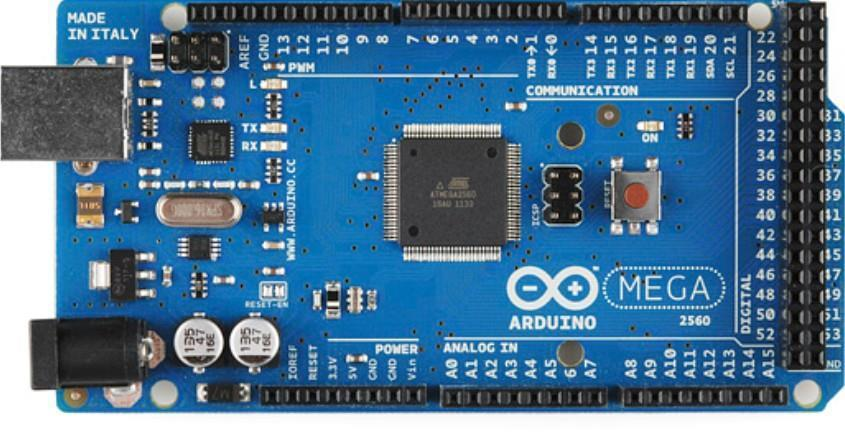
\includegraphics[width=1\linewidth]{arduino-mega}
				\caption{Arduino MEGA 2560}
				\label{arduino-mega}
			\end{figure}
	
		\subsection{Arquitectura}

			La \textbf{Figura \ref{esquemageneral}} refleja un esquema general de todos los componentes que interactúan entre sí y que hacen a la funcionalidad del sistema en su plenitud. Desde el desarrollo de una aplicación híbrida se realiza la conectividad entre el dispositivo móvil y la plaqueta Arduino. En propósito principal de la plaqueta Arduino es tomar las mediciones obtenidas por cada sensor conectado a la misma. La conectividad en el esquema planteado se realiza a través del módulo Bluetooth, de forma tal que la conexión se interpreta como una conectividad punto a punto y los datos son transferidos como un buffer de datos el cual debe ser interpretado por cada parte.

			\begin{figure}[h]
				\centering
				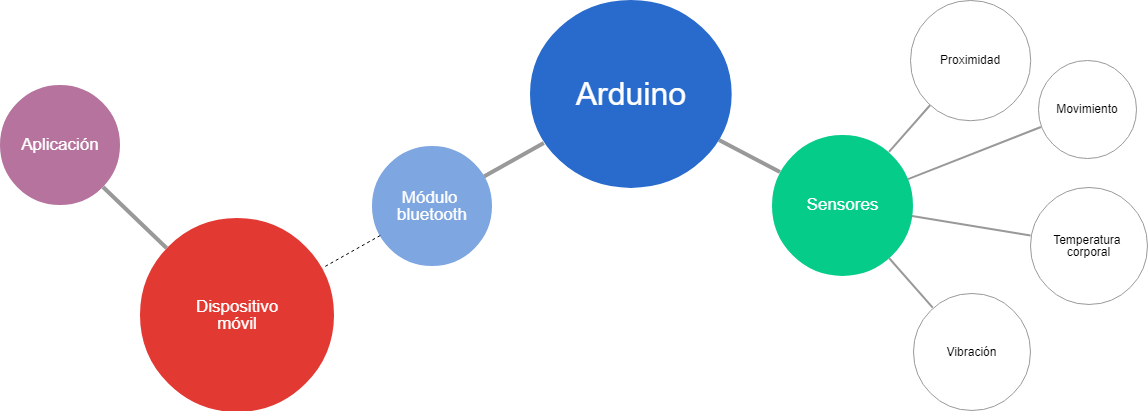
\includegraphics[width=1\linewidth]{esquemageneral}
				\caption{Esquema general de la arquitectura utilizada}
				\label{esquemageneral}
			\end{figure}

            \textbf{Ionic:}\\
			Ionic es un framework diseñado para el desarrollo de aplicaciones móviles híbridas, el cual se basa en Angular, Typescript, Javascript, CSS3 y HTML5. El concepto principal se basa en la traducción gráfica de todos los componentes visualizados en cada dispositivo móvil dependiendo la plataforma en la cual se encuentre, ya sea para Android o para iOS, cada componente utilizado tiene su representación gráfica acorde a la plataforma.

			Uno de los principales pilares que tiene Ionic es el de incorporar las librerías de Apache Cordova, la cual contiene toda la lógica, o motor principal, para traducir el código desarrollado independiente por cada plataforma. Es decir, Cordova contiene los desarrollos individuales, algunos desarrollados oficialmente y otros por grupos de desarrolladores de la comunidad que hacen su aporte, de los plugins que hacen a la funcionalidad de cada módulo del sistema operativo en cuestión. 

			En la \textbf{Figura \ref{ionic-angular-cordova}} se puede observar cómo interactúan los distintos componentes que hacen al desarrollo de la plataforma final distribuida para cada sistema operativo.

			\begin{figure}[h]
				\centering
				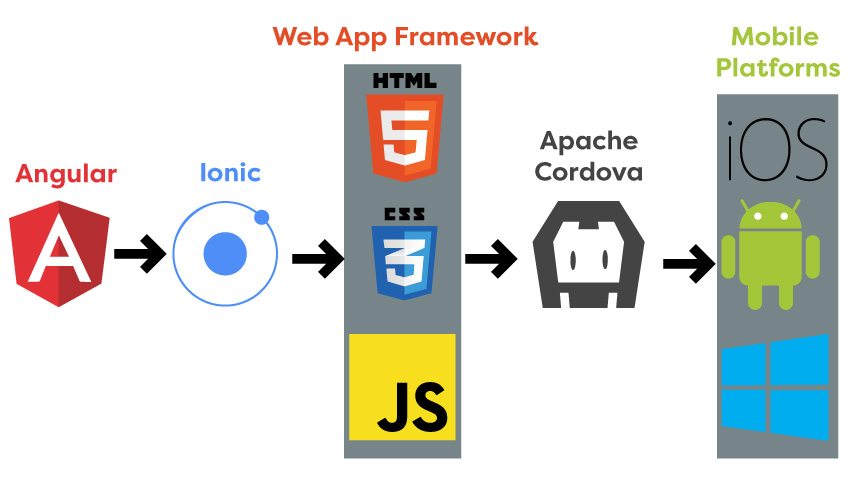
\includegraphics[width=1\linewidth]{ionic-angular-cordova.jpg}
				\caption{Componentes de la plataforma}
				\label{ionic-angular-cordova}
			\end{figure}

			En lo que respecta al desarrollo híbrido, el aplicativo final para cada plataforma, se traduce como un navegador web incorporado el cual es visualizado por el usuario final. Es por ello que el desarrollo principal está hecho sobre plataformas web. En la \textbf{Figura \ref{ionic-angular-cordova-webview}} se observa el componente WebView que interpreta los recursos incorporados y los lenguajes HTML, CSS y Javascript, dicho componente es el que simula un navegador web dentro del aplicativo final. \newpage

			\begin{figure}[h]
				\centering
				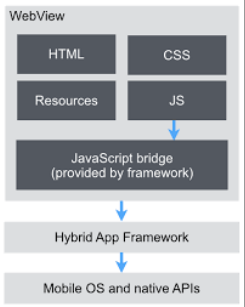
\includegraphics[width=0.6\linewidth]{ionic-angular-cordova-webview.png}
				\caption{Componente WebView}
				\label{ionic-angular-cordova-webview}
			\end{figure}
			

		\subsection{Conectividad inalámbrica}

			Existen distintos tipos de dispositivos y métodos de conectividad inalámbrica que pueden ser aplicados al sistema en cuestión. El abanico de posibilidades a implementar reside desde dispositivos Bluetooth, módulos WIFI o hasta incluso conectividad telefónica GSM que podría aprovecharse según el esquema en el cual se encuentre implementado el dispositivo o hacia donde quiera desarrollarse. Los ítems estudiados y que mejor se adaptan al dispositivo en cuestión corresponden a las siguientes posibilidades inalámbricas:\\

		    \textbf{Bluetooth:}
		
				El módulo bluetooth proporciona una conectividad de protocolo denominada como punto a punto, la cual se centra en emisión y recepción de información bidireccional a través de un buffer de datos. 
				El concepto denominado para el uso de ésta tecnología es WPAN, haciendo referencia al uso de una red inalámbrica de área personal, y sus características radican en la propagación de ondas de radiofrecuencia en la banda ISM de 2.4 GHz. 
				Su utilidad principal puede ser conocida como la conexión para la transferencia de información entre dos dispositivos celulares, por lo que en este caso se estudia como posibilidad para ser implementado en la conexión entre la placa Arduino y un dispositivo móvil para la visualización de datos y alertas.\\

			    \textbf{Wifi:}
				
				Se denomina conectividad Wifi a la posibilidad de conectar uno o varios dispositivos entre sí o a través de internet mediante distintos protocolos utilizados. Éste método de conectividad es ideal para la transferencia de información entre la placa Arduino y uno o más dispositivos móviles conectados a través de internet, los cuales pueden ser los dispositivos de los padres y/o tutores del bebé. 
				El protocolo Wifi a utilizar es conocido como TCP, el cual se conectaría a través de internet a un sistema en la nube o API, la cual se encarga de recolectar y almacenar la información suministrada por todos los sensores. El flujo de información en bidireccional por lo que también es posible tomar valores provenientes de algún dispositivo móvil para que desde Arduino realice alguna acción en caso de necesitarla.

	\section{Desarrollo}

		\textbf{Metodología de desarrollo:}\\
Dada la naturaleza de investigación de este proyecto, se sabía de antemano que se iba a trabajar a base de prueba y error para determinar la viabilidad de diferentes partes, tanto de hardware como de software. Los requerimientos y el alcance del proyecto van a cambiar de acuerdo a los resultados de las pruebas, por lo que se optó por proceder de la siguiente manera:

\begin{itemize}
    \item Etapa de investigación documental.
    \item Evaluación de tecnologías.
    \item Desarrollo de un prototipo.
\end{itemize}

El desarrollo de la APP fue llevado en paralelo a las pruebas de los sensores, ya que de ello depende el diseño de la misma y de los algoritmos que procesarán las mediciones.

\subsection{Evaluación de sensores}

Para este estudio se investigó, analizó y probó una variedad de sensores. Como se verá a continuación, no todos fueron seleccionados para el prototipo. Los sensores probados fueron: 

			\begin{itemize}
				\item Luz BH1750
				\item Vibraciones (Piezoeléctrico)
				\item Movimiento PIR-SR501
				\item Temperatura y humedad relativa ambiente
				\item Gases combustibles MQ-2
				\item Monóxido de carbono MQ-7
				\item Temperatura infrarrojo
				\item Proximidad
				\item Sonido
			\end{itemize}

Existe una amplia variedad de sensores disponibles en el mercado. Luego de una preselección, se hicieron pruebas individuales para determinar el comportamiento de cada uno de ellos.
Algunos sensores ofrecen mediciones en una unidad específica, con su error de medición para determinadas condiciones del ambiente. Otros sensores miden de forma amodal, con la posibilidad de realizar una conversión para obtener una unidad en particular.
En ambos casos, se presenta el problema de que el sujeto a sensorizar no es estático. El bebé se moverá dentro de la cuna y las mediciones se verán severamente afectadas por la variable distancia. Esto nos llevó a descartar un número de sensores, como se verá en las pruebas realizadas. Sin embargo, otros sensores son adecuados para medir la posición del bebé en la cuna e incluso determinar determinados comportamientos, como por ejemplo intentar trepar sobre una de las barandas o por el contrario, detectar una reducción de movimiento.
El conjunto de sensores ambientales fue más sencillo de seleccionar ya que se trabaja con la premisa de que la cuna del bebé estará bajo techo. 

Para observar el comportamiento de los sensores, se utilizó el software open-source TelemetryViewerv0.4. Este software muestra los datos leídos de un sensor en forma gráfica y en tiempo real, lo que permitió realizar las siguientes pruebas para cada sensor:

\textbf{Luz:} \\ 
El objetivo de este sensor es emitir una notificación cuando se detecta una fuente de luz que pueda estar afectando directamente a la cabeza del bebé, por lo que estará ubicado en la cabecera de la cuna.
El sensor fue fijado sobre una superficie plana y se observaron las mediciones con fuentes de luz desde diferentes direcciones. Se utilizaron luces dicroicas y luces LED. 
La curva generada por TelemetryViewer nos muestra que el sensor es extremadamente sensible a la dirección de la fuente de luz. Cualquier movimiento genera una variación en el gráfico. También se observó la diferencia entre una luz LED y una dicroica, independientemente de su potencia. La luz dicroica genera oscilaciones en el gráfico debido a la frecuencia de la corriente alterna, mientras que la luz LED presenta una curva suave (ver figura 1.1.1). 
La primer opción es disparar una notificación cuando el sensor, estando correctamente ubicado, alcance un determinado valor.
En caso de que no sea suficiente con establecer un valor arbitrario a partir del cual se emite la notificación, es necesario medir la luz ambiente deseada durante un periodo de tiempo para establecerla como valor norma.La App presentará un menú donde el usuario debe indicar que la iluminación medida en ese momento es la deseada. Mientras que el sensor tenga margen para medir mayor luz, el valor será aceptado y al medirse variaciones se disparará una notificación.
Si bien sería útil poder identificar la dirección de las fuentes de luz, ningún sensor es capaz de determinarla.\\

\textbf{Piezoeléctrico:}\\
Utilizamos varias unidades de este sensor. Originalmente adquirimos una unidad, y luego de las primeras pruebas lo encontramos sumamente útil. El sensor es extremadamente sensible a presiones e incluso vibraciones. La idea es ubicar una grilla de estos sensores por debajo de la manta donde el bebé descansa, y observando las mediciones de los diferentes piezoeléctricos poder indicar en qué posición se encuentra el bebé. Fácilmente puede registrarse cuánto tiempo permanece en cada posición, si se encuentra acostado o de pie, pero por sobre todas las cosas nos da la posibilidad de detectar episodios epilépticos, falta de movimiento y posibles posiciones incómodas o contraindicadas. A mayor número de sensores, mayor precisión se tendrá. A modo de prueba de concepto, implementamos solamente cuatro sensores.
Por otro lado, ubicamos otras unidades debajo de las barandas de la cuna, pudiendo enviar notificaciones cuando el bebé se apoye sobre ellas y intente trepar fuera de ella.\\

\textbf{Movimiento:}\\
Las pruebas mostraron que el sensor mide únicamente la existencia o inexistencia de movimiento. No sirve para medir distancias ni ubicar a objetos en el espacio.
Si bien a primera vista parece ofrecer poca información, su sensibilidad es muy alta y su rango es suficiente para el tamaño de una cuna. Puede usarse en conjunto con los sensores piezoeléctricos para aumentar la precisión de las notificaciones, ya que pequeñas vibraciones pueden activar a los piezoeléctricos pero únicamente el movimiento del bebé activará al sensor de movimiento.
Incorporar sensores de movimiento en el perímetro de la cuna ayuda a diferenciar entre una persona adulta apoyándose sobre una baranda de cuando el bebé lo hace, ya que en el primer caso se estarían activando los sensores de movimiento perimetrales.
La App permitirá activar y desactivar las notificaciones para los sensores de movimiento perimetrales.
Alcance del sensor en distancia y ángulo.\\

\textbf{Temperatura y Humedad Relativa ambiente:}\\
La App muestra ambos datos en tiempo real y el usuario podrá, opcionalmente, definir un valor máximo y mínimo a partir del cual se emitirán las notificaciones.\\
El sensor tiene la siguiente precisión:
\begin{itemize}
    \item Humedad Relativa a 25\textordmasculine C:  5\%
    \item Temperatura: a 25\textordmasculine C:  2\textordmasculine C
\end{itemize}

Como sensor complementario, hubiese sido de gran utilidad medir corrientes de aire en el ambiente. Si el sensor de Temperatura está tapado o bloqueado, no se verá afectado por la corriente de aire pero el bebé sí, lo que dispararía una notificación. Lamentablemente no encontramos este tipo de sensores en el mercado Argentino.\\

\textbf{Gases combustibles:}\\
El sensor MQ-2 detecta Hidrógeno, monóxido de carbono, gas Licuado, gas butano, gas metano, gas propano, alcohol y humo. Pero es más sensible al gas licuado, butano, metano, alcohol e hidrógeno. Si bien muchos de estos gases es poco probable que estén presentes en el ambiente de un bebé, el sensor nos es útil para detectar gas natural de red y concentraciones de alcohol, que al ser muy utilizado en higiene y medicina, puede acumularse por falta de ventilación. 
Se hicieron pruebas informales con alcohol, monóxido de carbono, gas de red y humo. Decimos que son pruebas informales porque no fueron en entorno de laboratorio y cada uno de esos gases estaba contaminado por el aire del ambiente. Sin embargo la consideramos una prueba válida ya que simula las condiciones en las que operará el sensor en la vida real. Los resultados fueron positivos, el sensor mostró un tiempo de respuesta más que suficiente para todos los gases aunque el monóxido de carbono será doblemente verificado con un sensor específico para ese gas, ya que lo consideramos crítico por su toxicidad.\\

\textbf{Monóxido de carbono:}\\
El sensor MQ-7 es comercialmente conocido para detectar monóxido de carbono. Sin embargo, fue probado a la par del sensor MQ-2 y respondió a todos los gases con igual sensibilidad. Según la ficha técnica \cite{refmq7} el MQ-7 es particularmente sensible al monóxido de carbono, por lo que es el primer sensor de donde tomamos la medición para este gas. Igualmente se toma la lectura del MQ-2 como redundancia. La App disparará alertas al detectar niveles de gases elevados, aunque no pueda identificarse específicamente que tipo de gas es.\newpage

\textbf{Temperatura Infrarrojo:}\\
El objetivo de este sensor era medir la temperatura del bebé sin entrar en contacto con su piel. Si bien sabíamos de antemano que no iba a ser una medición exacta, hubiese servido al menos de manera referencial, para detectar cambios bruscos en las mediciones y cruzar los datos con las lecturas del sensor de Temperatura y Humedad ambiente.
Lamentablemente, el alcance de este sensor es insuficiente para este proyecto. Sin superar los 25cm, las mediciones varían muchísimo para un mismo objeto a diferentes distancias, haciéndolo muy poco confiable. Especialmente cuando se trata de un bebé que se moverá de manera impredecible.
Sin conocer la distancia entre el sensor y el bebé, y sin poder ajustar esta distancia para que se mantenga dentro del rango ideal de medición para este sensor, no hay forma alguna de darle algún uso.
Por estas razones, la lectura de temperatura del bebé queda descartada.\\

\textbf{Proximidad:}\\
Este sensor podría haber sido usado como alarma perimetral. Iba a estar ubicado en todos los puntos donde el bebé pudiera salir de la cuna, pero falló la primer prueba de alcance. Al no poder detectar movimiento a más de 30cm de distancia, no alcanza a leer ni la mitad de la baranda de una cuna promedio. 
Por esta razón se optó por utilizar un sensor piezoeléctrico en conjunto con sensores de movimiento para determinar si el bebé está intentando salir de su cuna. Si bien es llamado sensor de proximidad, no mide a qué distancia fue detectado el objeto. Hicimos pruebas para confirmarlo y utilizando TelemetryViewer confirmamos que únicamente envía señal alta cuando un objeto interrumpe la emisión infrarroja del sensor y señal baja cuando nada la distorsiona. De haber podido leer la distancia a la que se encuentra el objeto, se podría haber implementado para aumentar la precisión de medición de movimiento del bebé, así como su ubicación en la cuna y sobre los sensores piezoeléctricos.\\

\textbf{Sonido:}\\
Sin duda, el sensor más difícil de probar y calibrar. El objetivo es enviar notificaciones cuando se midan sonidos fuertes dentro del ambiente donde está el bebé.
Realizamos pruebas utilizando TelemetryViewer para familiarizarnos con el comportamiento del sensor. Observando las curvas generadas, notamos que se requiere de ruidos muy fuertes para ver cambios grandes en las mediciones. Si bien las mediciones son amodales, daremos un rango de 0 a 1023 para facilitar la comprensión de las pruebas. 
En un ambiente silencioso, el sensor oscila entre 5 10 puntos de medición. Ruidos provenientes de la calle con una ventana abierta, como el tránsito de un colectivo y automóviles, se miden con variaciones de hasta 25 puntos. Sin embargo, un grito humano es medido con hasta 100 puntos, mientras que un aplauso o un golpe seco son lo único que disparan al máximo las mediciones del sensor.
Para conocer aún más su comportamiento, utilizamos un generador de frecuencias con el que recorrimos el rango audible por humanos manteniendo volumen y distancia constantes. El resultado es una mayor medición para frecuencias de rango medio, obteniendo una mayor amplitud en el gráfico del TelemetryViewer cuanto más cerca se encuentra la fuente sonora. 
Estas pruebas son consideradas positivas. La cercanía del bebé al sensor, el volumen de su llanto y su duración nos hacen posible distinguirlo del ruido ambiente y sonidos provenientes de la calle.\newline

Luego de las pruebas, se definieron los siguientes sensores a utilizar en el sistema:

			\begin{itemize}
				\item Luz
				\item Vibraciones (Piezoelectrico)
				\item Movimiento
				\item Tempreatura y humedad relativa ambiente
				\item Gases combustibles
				\item Monóxido de carbono
				\item Sonido
			\end{itemize}


\subsection{Aplicación}

Como se mencionó antes, el usuario interactuará con el sistema a través de una App. Podrá definir valores máximos y mínimos a partir de los cuales recibirá alertas, activar y desactivar sensores individualmente y ver estadísticas.
En estado de prototipo, la pantalla inicial de la aplicación solicita la conexión Bluetooth con el dispositivo. Una vez establecida, se pueden ver las lecturas de cada sensor en la pantalla principal (Figura 5).
El side menu ofrece opciones de configuración, donde el usuario podrá activar o desactivar cada sensor y definir los umbrales para las notificaciones(Figura 6).


			\begin{figure}[h]
				\centering
				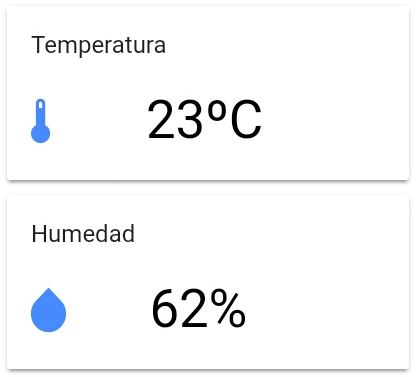
\includegraphics[width=0.3\linewidth]{lecturas_cortadas.png}
				\caption{Vista de sensores para el usuario.}
				\label{Vista de sensores para el usuario.}
			\end{figure}

			\begin{figure}[h]
				\centering
				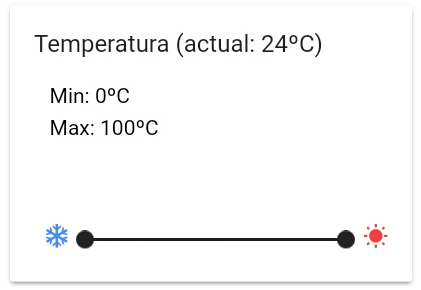
\includegraphics[width=0.5\linewidth]{parametros_cortada.png}
				\caption{Parametros para un sensor.}
				\label{Parametros para un sensor.}
			\end{figure}

Se hicieron pruebas de conectividad WiFi. El proyecto requiere una alta frecuencia de envío de mensajes desde el dispositivo hacia la aplicación para obtener lecturas en tiempo real. Mediante la conexión WiFi, no es posible mantener este envío de datos sin pérdidas o retrasos. Perder la habilidad de lectura de sensores en tiempo real es completamente inadmisible, inclusive para una versión de prototipo, por lo que optamos por la conectividad Bluetooth. Adicionalmente, para la conectividad WiFi es necesario 115200 baudios, mientras que para Bluetooth es suficiente con 9600. Dado que Arduino funciona con una única configuración de baudios, no nos fue posible implementar ambas opciones de conectividad en simultaneo con el hardware actual.\\

El código en Arduino se limita a la lectura de datos de los sensores y al envío de ellos mediante el módulo Bluetooth.\\ 
La transmisión de datos mediante Bluetooth requirió el desarrollo del siguiente protocolo: 
Desde Arduino se envían 4 caracteres para la identificación de cada sensor, seguido con el valor transmitido, concatenado con un caracter ‘|’ que indica el fin de los datos de cada sensor. Todo esto es transmitido con un buffer de datos que es interpretado por la aplicación. Se puede apreciar la lectura de los sensores y el armado de la cadena en las imagenes 7 y 8. Una vez que la aplicación recibe los datos, se procesan para decidir si se enviarán alertas o no.

			\begin{figure}[h]
				\centering
				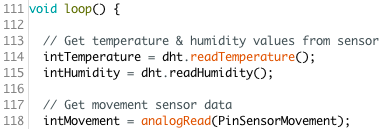
\includegraphics[width=0.8\linewidth]{codigo_arduino_lectura_cortada.png}
				\caption{Codigo Arduino, lectura de sensores.}
				\label{Vista de sensores para el usuario.}
			\end{figure}

			\begin{figure}[h]
				\centering
				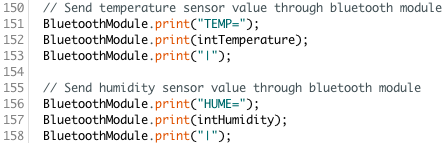
\includegraphics[width=0.8\linewidth]{codigo_arduino_protocolo_cortada.png}
				\caption{Codigo Arduino, armado de cadena}
				\label{Parametros para un sensor.}
			\end{figure}

%\newpage


		\subsection{Materiales}
        Los materiales utilizados para el desarrollo del prototipo son:
		        \begin{itemize}
			\item Arduino Mega 2560
			\item PC
			\item Sensor luz: BH1750
			\item Sensor Gases Combustibles: MQ-2
            \item Sensor Gases secundario: MQ-7
            \item Sensor Piezoelectrioco x5: AA2758
            \item Sensor Movimiento x2: PIR SR-501
            \item Sensor Temperatura y Humedad ambiente: DHT11 
            \item Sensor Sonido: KY-038
            \item Modulo Bluetooth: HC-06
            \item Protoboard
            \item Modulo WiFi: esp-11e
		\end{itemize}
		Insumos
		\begin{itemize}
		
    		\item Cables Dupont m-m, m-h
    		\item Bateria 9v
    		\item Cable adaptador Bateria - Jack Arduino
    		\item Adaptadores m-m, m-h y h-h para cables Dupont
		
		\end{itemize}

	\section{Conclusión}

Arcangel aprovecha la tecnología comercialmente accesible de hoy en dia para tomar datos sensoriales del bebé y del ambiente donde descansa. Estos datos resultan útiles para las personas a cargo del cuidado de los pequeños. 
Si bien el avance de la tecnología hará que se lancen nuevos sensores al mercado, la modularización del sistema nos da gran libertad para reemplazarlos y probar nuevas versiones. La elección de Arduino Mega para el prototipo nos da esta flexibilidad, ya que a lo que sensores respecta es una solución sobredimensionada.
Una vez lograda la comunicación entre Arduino y la APP, pudimos procesar los datos para identificar posibles situaciones de riesgo y emitir alertas acordes.
En lo que a software respecta, hay lugar para campos como Inteligencia Artificial que permitirán mayor precisión a la hora de emitir notificaciones, mejorando la confiabilidad del sistema.
El mayor desafío de Arcangel es la comunicación en tiempo real entre el dispositivo y la aplicación móvil. Para mejorar su performance y confiabilidad, no se descarta una solución utilizando Raspberry pi en lugar de Arduino.


	\section{Líneas futuras de investigación}

		\begin{itemize}
			\item Detección de necesidad de cambiar al bebé.
			\item Implementar inteligencia artificial para aumentar la precisión del sensor de sonido a la hora de detectar el llanto del bebé.
			\item Implementar inteligencia artificial para detectar ataques epilépticos.
			\item Incorporar una solución utilizando Raspberry PI.
		\end{itemize}
		
	\bibliographystyle{IEEEtran}	
	\bibliography{bibliografia}
	\newpage
	
	\section{CV}
	
%	\begin{wrapfigure}{l}{0.25\textwidth}
%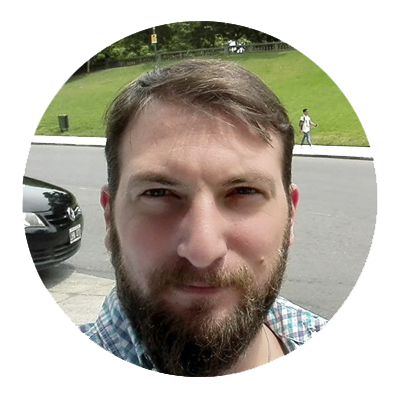
\includegraphics[width=0.6\linewidth]{diego.png} 
%\label{fig:subim1}
%\end{wrapfigure}

\begin{wrapfigure}{l}{0.15\textwidth}
    \centering
    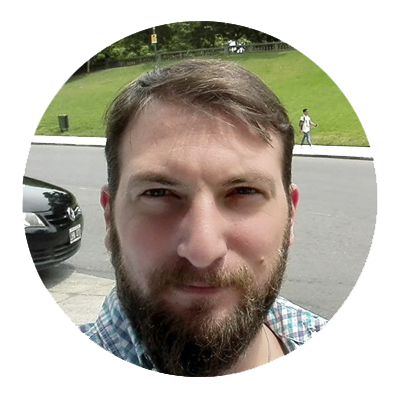
\includegraphics[width=0.15\textwidth]{diego.png}
\end{wrapfigure}
        
        Diego Ariel Bertolini
        
        www.diegobertolini.com
        
        Octubre 2015 / Actualidad:
        
        Consultor Business Intelligence
        
        Actualmente llevo a cabo la tarea de mantenimiento de estructuras de datos, desarrollo de tableros departamentales en QlikView y Qlik Sense. Creación e implementación de documentos y extensiones de objetos utilizados en las aplicaciones. Administración básica de servidores y consola de ejecución de tareas de Qlik, mashups y objetos embebidos en páginas web.
        
        Data IQ (IT Deals S.A.)
        Av. del Libertador 5478 CABA
        www.dataiq.com.ar
        Desarrollo y mantenimiento de tableros de control
        QlikView
        Qlik Sense
        
        Junio 2006 / Octubre 2015:
        Previo a la consultoría BI he desarrollado la tarea help desk y de analista programador en distintas empresas, basados en el desarrollo web y aplicaciones de escritorio.
        
        \begin{itemize}
			\item OCA S.R.L.
			\item Ideas in Motion S.R.L.
			\item Teceng Gaming S.A.
			\item Universidad Nacional de La Matanza
            \item Codes S.A.
		\end{itemize}
        
        Las tecnologías utilizadas fueron:
        
        \begin{itemize}
			\item SQL Server
			\item PostgreSQL
			\item MySQL
			\item Net C\# 
            \item Crystal Reports
            \item PHP
            \item Javascript
            \item HTML
		\end{itemize}
		\vspace{10mm}
		\newpage
		Juan Manuel Alvares: Nacido en Buenos Aires, Argentina, el 17 de marzo de 1988.
Este trabajo es su última asignatura para completar la carrera de Ingeniería en Informática, en la Universidad de Palermo.
Su experiencia laboral se basa en mantenimiento de oficinas, instalaciones de red y recientemente tuvo la oportunidad de realizar el desarrollo de una aplicación Java como solución de software para una empresa en la cual realizó su práctica profesional supervisada.
Lenguajes conocidos: 
\begin{itemize}
			\item Java
			\item PL/SQL
			\item HTML
			\item CSS 
            \item C
		\end{itemize}

    

		
\end{document}